\documentclass[12pt]{article}
% Margin fixes
\oddsidemargin -0.5in
\evensidemargin -0.5in
\textwidth 7.25in
\topmargin 0.0in

\headheight 0.0pt
\headsep 0.0pt
\voffset 0.0pt
\textheight = 9.0in
\usepackage{amsmath,amssymb,graphicx,float}

\title{Electron Spin Resonance}
\author{Nathan Grouse\\Lisa Tran}

\newcommand{\eV}{\text{eV}}
\newcommand{\V}{\text{V}}
\newcommand{\A}{\text{A}}

% Start the document!
\newcommand{\documentname}{\textsl{Article}}
\begin{document}
\maketitle

\section{Introduction}
\indent \indent An oscillating magnetic field is used to induce transitions between energy levels taken on by electrons in this field.

\subsection{Apparatus}
\indent \indent Helmholtz coils wired in parallel, a multimeter to measure the current in the coils, a power source provides a DC voltage with a possible modulation voltage, and an oscilloscope are used.

\begin{figure}[H]
\centering
\hspace{-0.0in}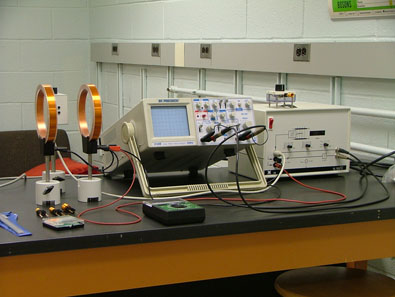
\includegraphics[scale=0.90]{apparatus.png}
\end{figure}

\section{Theory}
\indent \indent Spin angular momentum:
\[\vec{S} = sqrt{s(s+1)}\frac{h}{2\pi} , \]
\indent where$s = \frac{1}{2}$ is the spin quantum number. This makes sense considering the half integer multiples of Planck's constant. \\

The spin angular momentum is related to the magnetic moment:
\[ \vec{\mu} = -(g_s \mu_B \vec{S})/\frac{h}{2\pi} \]
\indent Meaning magnetic moments also come in the same multiples as the spin angular momentum. $g_s$ is the g-factor and its value depends on the particle being described. $g_p_r_o_t_o_n = 5.586$, $g_e_l_e_c_t_r_o_n = 2.0023$, and $g_n_e_u_t_r_o_n = -3.826$. \\

\indent In a magnetic field that points in one direction, apparently the spin angular momentum can only have projections onto the respective axis, resulting in two values for the spin magnetic moment:
\[S_z = \hbar m_s ,\]
\indent where $m_s = \pm \frac{1}{2}$ are the possible values for the magnetic spin quantum number. So the spin magnetic moment also takes on two different values in one dimensional magnetic fields:
\[\mu_z = -(g_s \mu_B S_z)/\hbar = \pm \frac{1}{2}g_s \mu_B  .\]
\indent Two possible energy levels are defined by this too:
\[U = -\vec{\mu}\cdot \vec{B} = \pm \frac{1}{2}g_s \mu_B B , \]
\[\Delta E = h\nu = g_s\mu_B B .\]
\indent Where $\nu$ is the minimum frequency of radiation that would induce or be emitted during a change of state for a particle in one dimension, derived from the Einstein relation.

\section{Data}
\begin{figure}[H]
\centering
\hspace{-0.0in}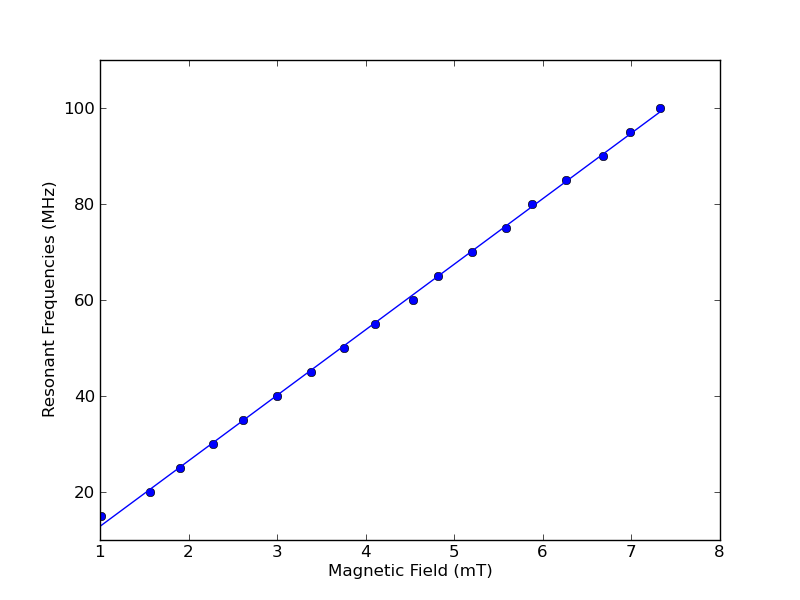
\includegraphics[scale=0.60]{Plot1.png}
\caption {$\nu$ = $\frac{g \mu_B}{h}$ B, Slope = 13.66 $\frac{MHz}{mT} \label{fig:setup}}
\end{figure}

\section{Calculations}
\indent \indent Measuring g:
\[\nu =  $\frac{g \mu_B}{h}$ B\]
\[\frac{g \mu_B}{h}(10^9) = 13.66 \frac{MHz}{mT} = 1.366 x 10^1^0 \frac{Hz}{T} \]
\[g = (1.366 x 10^1^0)\frac{h}{\mu_B} = .975 \]

Measuring $\delta$B:
\[\delta W = 1.2 cm\]
\[I_m_o_d_,_r_m_s = .33 A \]
\[I_m_o_d_,_p_-_p = 2\sqrt{2} I_m_o_d_,_r_m_s = .93 A \]
\[\delta (2I_0) = I_m_o_d_,_p_-_p \frac{\delta W}{10} = .011 A\]
\[\delta B = 2.115 \delta (2I_0) = .0237 mT \]

\section{Error Analysis}
\indent \indent The value of \delta B is within the designated range of line widths quoted in the literature. I won't check it's percent error because the line width depends on the solvent in which the sample has recrystallized. The uncertainty in the resonant frequency readings is $\pm$ .05 MHz, as indicated by the decimal accuracy of the machine's readings. The uncertainty in the current readings is $\pm$ .005 A, as indicated by the decimal accuracy of the multimeter. Uncertainty propogated linearly through calculating values of the magnetic field between the coils from current:
\[B_m_a_x = 2.115(2(I_0 + .005 A)) = B + .02115 mT \]
\[B_m_i_n = 2.115(2(I_0 - .005 A)) = B - .02115 mT \]
\[\delta B = \pm .02115 mT \]

\indent Percent Error on g:
\[\frac{|2.0023 - .975|}{2.0023} = 51.3 \% \]

\section{Conclusion}
\indent \indent The numbers I obtained for both g and $\delta$B seem reasonable and consistent with the accepted value. I did see what I expected to see in terms of the resonance curves.

\section{Questions}
\indent \indent 1. The manufacturer designed this experiment with the coils connected in parallel. A series connection would be better. Why? \\
\indent If the inductances of two coils located in each others magnetic field are not equal, this can cause short circuiting. \\
\indent 2. The p-p modulation current $\delta$(2I_0) for the half-width $\delta$B is obtained from:
\[\delta (2I_0) = I_m_o_d_,_p_-_p \frac{\delta W}{10} \]
\indent Where does the divisor 10 come from? \\
\indent It changes the value of $\delta$W so that it represents meters. \\
\indent 3. In the method given for measuring $\delta$B, the scope controls are not used in a calibrated mode. Why is this OK? \\
\indent We account for it by dividing $\delta$W by 10. \\
\indent 4. Why is the multimeter set for DC amperes for measring g and for AC amperes for measuring the line width? \\
\indent Not sure. Maybe because AC amperes are required for generating p-p values. \\
\indent 5. Is there an RF electric field associated with the RF coil? If so, make a sketch of what the fields look like. \\
\indent I think there is an RF electric field but I don't know what it looks like.

\end{document}